Maven \`e un tool per l'automazione della compilazione usato principalmente per progetti Java.  Maven a ronta due aspetti della compilazione del software:
per prima cosa descrive come il software dev'essere compilato, e poi descrive le sue dipendenze.  A di erenza di tool pi\`u datati come Ant, utilizza convenzioni per la procedura di compilazione, in cui vanno speci cate solamente le eccezioni.  La configurazione del progetto va e ettuata in un  le XML, in cui viene descritto il progetto, le sue dipendenze, l'ordine di compilazione, le directory sorgenti, ed eventuali plugin.  Maven contiene target prede niti per task ben de niti, come ad esempio la compilazione e la pacchettizzazione.  Durante la risoluzione delle dipendenze, Maven scarica automaticamente le librerie e i plugin necessari da uno o pi\`u repository, e salva il tutto in una cache locale, che  pu\`o  essere  anche  aggiornata  con  artefatti  provenienti  da  progetti  locali.
Maven pu\`o anche essere usato per gestire progetti scritti in C#, Ruby, Scala, e altri linguaggi.  Progetti alternativi come Gradle e
SBT (Scala Build Tool) non utilizzano XML ma mantengono i concetti chiave
introdotti da Maven.
I  progetti  Maven  vengono  configurati  tramite  un  Project  Object  Model (POM) file.  Generalmente, questa configurazione comprende il nome del progetto e le dipendenze su altri progetti.  Si possono anche configurare fasi individuali del processo di compilazione, implementate tramite plugin.  Ad esempio, si pu\`o configurare il plugin del compilatore in modo che venga utilizzata una versionefispeci ca di Java, oppure specificare che si vuole ottenere il pacchetto anche se alcune unit\`a di test falliscono.  I progetti pi\`u grossi dovrebbero essere suddivisi in diversi moduli (sottoprogetti), ognuno con il proprio POM, collegati ad un POM radice attraverso il quale si possono compilare tutti i moduli con un unico comando.  I  le POM possono anche ereditare la loro configurazione da altri  le POM. Di default, tutti i POM ereditano dal POM radice.  Il POM radice fornisce la configurazione di default, speci cando ad esempio le cartelle sorgente, i plugin, e cos\`i via.
La maggior parte delle funzionalit\`a di Maven \`e fornita dai plugin.  Esistono plugin per compilare,  testare,  e gestire i sorgenti,  avviare un web server, generare  le di progetto Eclipse, e molti altri ancora. I plugin vengono speci cati e configurati nell'apposita sezione del  le POM. Alcuni plugin di base sono inclusi di default in ogni progetto, con ragionevoli impostazioni di default.  Tuttavia la procedura risulterebbe scomoda se si dovesse ad ogni compilazione invocare ogni goal manualmente.  Per questo motivo Maven introduce  il  concetto  di  lifecycle,  ovvero  insiemi  di  goal  lanciati  in  modo
sequenziale.
La gestione delle dipendenze \`e una caratteristica chiave di Maven, e si fonda su un sistema che identi ca artefatti come librerie o moduli.  Le dipendenze dirette di un progetto vengono speci cate nel suo POM, ma vengono valutate e scaricate anche tutte le dipendenze transitive, che vengono poste nel repository locale.  Di default viene utilizzato il Maven 2 Central Repository per la ricerca delle librerie,  ma si possono configurare repository esterni all'interno del POM.
\begin{figure}[!htb]
\centering%
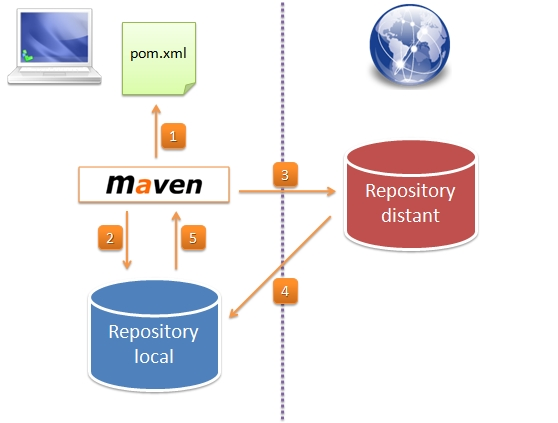
\includegraphics[scale=0.8]{maven.jpg}%
\caption{Maven}\label{fig:maven}%
\end{figure}